\documentclass[12pt]{article}
\usepackage{mathtools}
\usepackage{float}
\usepackage{tikz}
\usepackage{graphics}
\usepackage{refstyle}
\usepackage{subfig}
\usepackage{graphicx}
\graphicspath{{/storage/self/primary/Download/latex/image}}
\begin{document}
\title{\textbf{PROBABILITY}}
\date{}
\maketitle
\begin{enumerate}
    \item If $A$and$B$ are two events such that $P(A/B)=2 \times P(B/A)$ and $P(A)+P(B)=\frac{2}{3}$,then $P(B)$ is equal to
    \begin{enumerate}
        \item $\frac{2}{9}$
        \item $\frac{7}{9}$
        \item $\frac{4}{9}$
        \item $\frac{5}{9}$
    \end{enumerate}
    \item
    \begin{enumerate}
        \item Two balls are drawn at random one by one with replacement from an urn containing equal number of red balls and green balls.Find the probability distribution of number of red balls. Also,find the mean of the random variable.
        \item A and B throw a die alternately till one of them gets a `6' and wins the game. Find their respective probabilities of wining,if A starts the game first.
    \end{enumerate}
   \item Recent studies suggest that roughly $12\%$ of the world population is left handed.(\figref{fig1})\\
\begin{figure}[H]
       \centering
       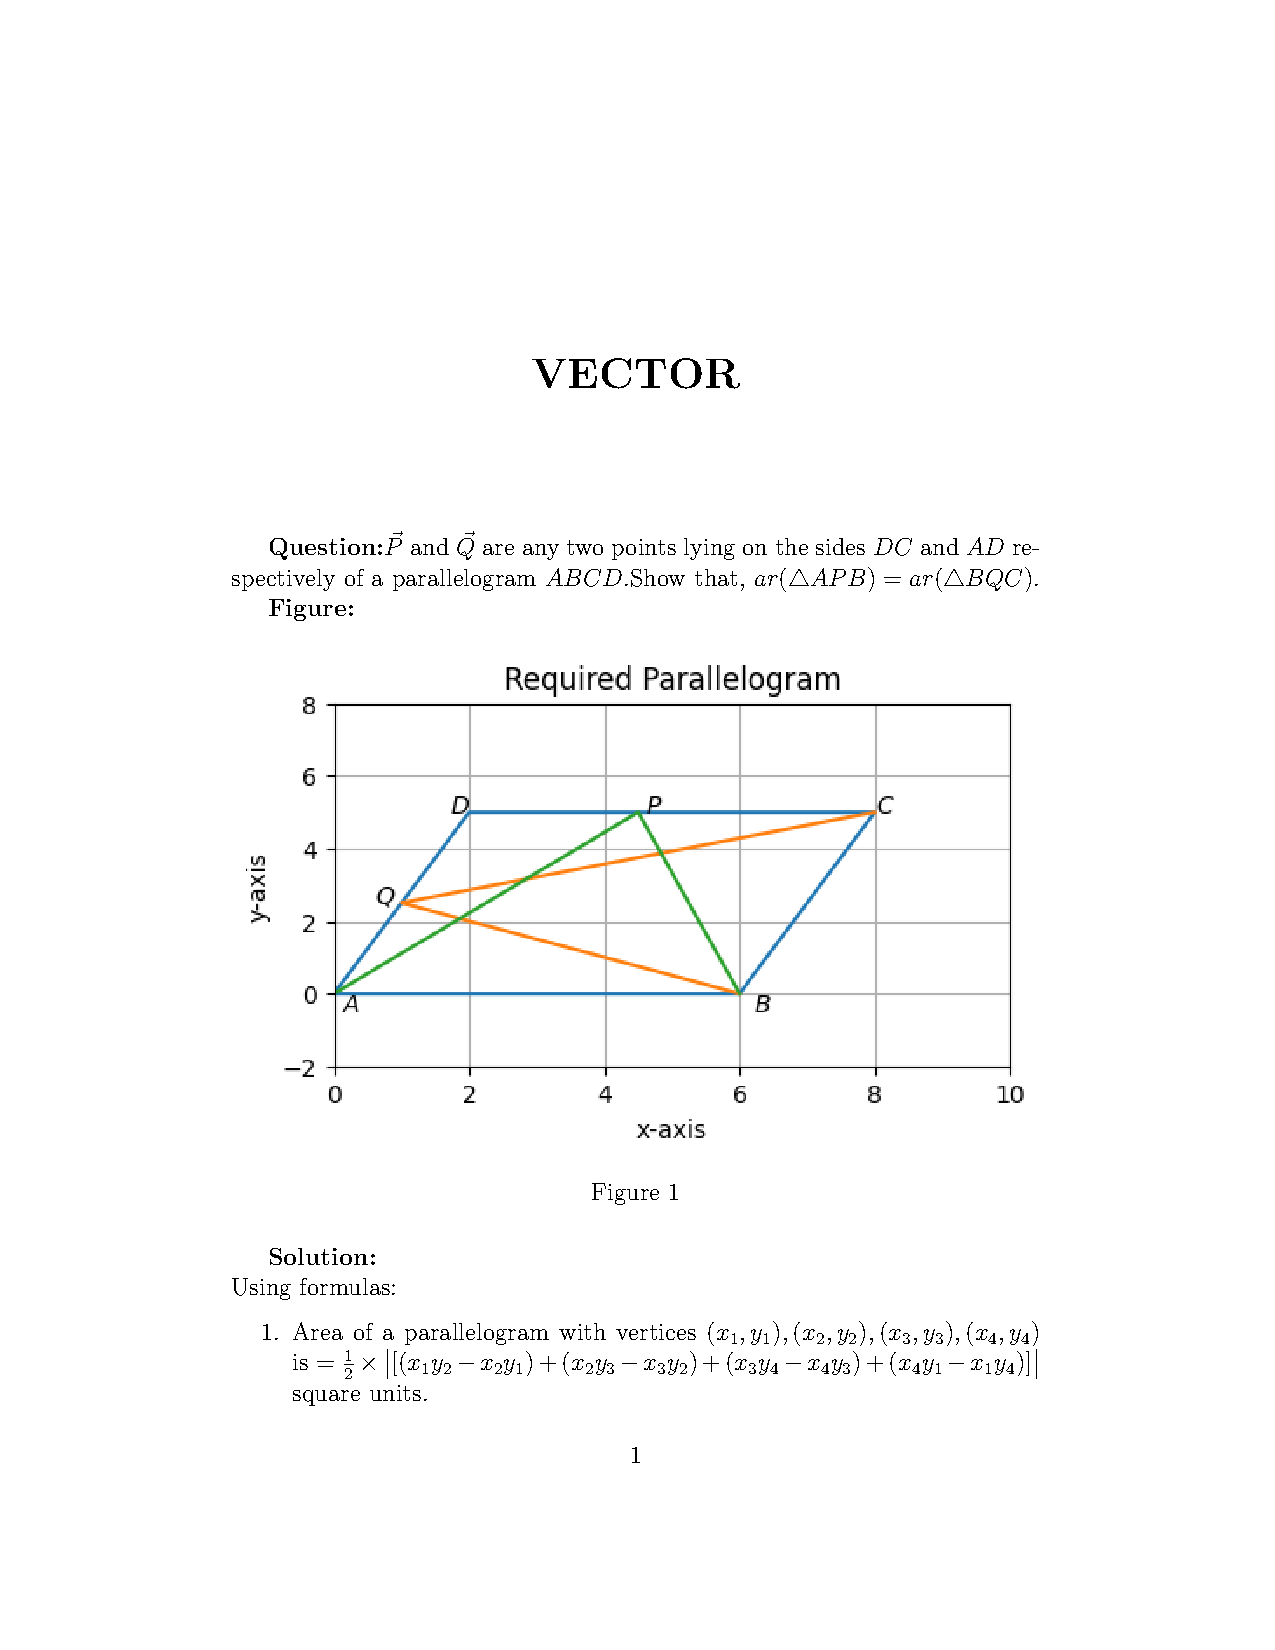
\includegraphics[width=\columnwidth]{image/1.png}
       \caption{}
       \label{fig:fig1}
\end{figure}
   Depending upon the parents,the chances of having a left handed child are as follows:\\
   
       A: When both father and mother are left handed:\\ Chances of left handed child is 24\%.\\
       B: When father is right handed and mother is left handed:\\ Chances of left handed child is 22\%.\\
       C:  When father is left handed and mother is right handed:\\ Chances of left handed child is 17\%.\\
       D:  When both father and mother are right handed:\\ Chances of left handed child is 9\%.\\
   Assuming that$P(A)=P(B)=P(C)=\frac{1}{4}$ and $L$ denotes the event that child is left handed.
   \begin{enumerate}
       \item Find $P(L/C)$
       \item Find $P(\bar L/A)$
       \item \begin{enumerate}
           \item Find $P(A/L)$
           \item Find the probability that a randomly selected child is left handed given that exactly one of the parents is left handed.
       \end{enumerate}
   \end{enumerate}
\end{enumerate}
\end{document}


